\documentclass[12pt]{article}
\usepackage[utf8]{inputenc}
\usepackage[T1]{fontenc}

\usepackage{bm}							% bold math symbols
\usepackage{amsmath}					% equation formatting
\usepackage{amssymb}					% equation symbols
\usepackage{mathtools}					% amsmath extension, symbols
\usepackage{siunitx}					% SI units package
\usepackage{caption}					% extended caption functionality
\usepackage{subcaption}					% provides subcaptions
\usepackage{graphicx}					% images
\usepackage{xcolor}						% driver-independent colors
\usepackage{wrapfig}					% figure wrapping
\usepackage{tikz}						% portable graphics format creator
\usetikzlibrary{decorations.pathreplacing}

\usepackage[margin=1in]{geometry}		% document layout package

\usepackage[notes,backend=biber]{biblatex-chicago} % citation styling
\usepackage[english]{babel}				% language package
\usepackage[autostyle=true]{csquotes}	% extended quotation functionality
\usepackage{hyperref}					% hypertext support

\usepackage{setspace}					% easy text spacing
%\usepackage{newtxtext,newtxmath} 		% times new roman, more up to date

% Standard ihat and jhat are not implemented by default.
% This provides the ihat and jhat without the dot at the top.
% Is basic implementation, does not work with mathptmx
%\newcommand{\ihat}{\mathbf {\hat \imath}}
%\newcommand{\jhat}{\mathbf {\hat \jmath}}

% Declare bibliography as the 'references.bib' file
\bibliography{references}

% Set doublespacing
\doublespacing
%\renewcommand{\baselinestretch}{1.5}

% Custom text formatting
\setlength{\parindent}{0pt}
\setlength{\parskip}{1em}

% Renaming the 'Contents' field to 'Table of Contents'
\addto\captionsenglish{ % required by babel
	\renewcommand{\contentsname}{Table of Contents}
}

% implementation of a unit vector as given by 'egreg' from tex.stackexchange.com 
% https://tex.stackexchange.com/questions/188775/how-to-type-a-particular-kind-of-unit-vector
\newcommand{\uveci}{{\bm{\hat{\textnormal{\bfseries\i}}}}}
\newcommand{\uvecj}{{\bm{\hat{\textnormal{\bfseries\j}}}}}
\DeclareRobustCommand{\uvec}[1]{{%
		\ifcat\relax\noexpand#1%
		% it should be a Greek letter
		\bm{\hat{#1}}%
		\else
		\ifcsname uvec#1\endcsname
		\csname uvec#1\endcsname
		\else
		\bm{\hat{\mathbf{#1}}}% This really is the only important thing
		\fi
		\fi
}}

\newcommand{\bvec}[1]{\bm{\mathbf{#1}}}

\captionsetup[figure]{font=small,justification=centering}

\allowdisplaybreaks

\begin{document}
	\begin{titlepage}
	\begin{center}
		\vspace*{\fill}
		
		The Mathematics behind Lagrange Points
		
		\vspace*{1.0cm}
		Word Count: \#\#\#\#
		
		\vfill
		
		Julian Joaquin\\
		Mathematics Internal Assessment\\
		Professor\\
		Date
		
		\vspace*{\fill}
		
	\end{center}
\end{titlepage}
	
	\tableofcontents
	
	\newpage
	
	\section{Introduction}
	
	In this day and age, the aerospace industry has become a vital component of the global economy.
In a publication by the Organisation for Economic Co-operation and Development, the space economy plays a key role in the globalization and digitization of the modern world, with space activities making crucial contributions to the social, economic, and scientific aspects of society\autocite{c5996201-en}.
With an increasing investment for spaceflight, there is future need to develop infrastructure that can facilitate the growing space sector, which includes the understanding of 
	
	\section{Finding the Lagrange Points}
	
	We will be determining the collinear Lagrange points from a rotating frame of reference relative to a circular orbit of Earth.
This simplifies the solution to a single dimension which bisects the Sun and Earth. % ELABORATE

\vspace*{0.5cm}
\begin{figure}[!h]
	\centering
	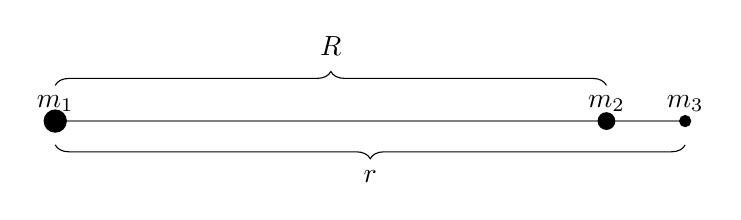
\begin{tikzpicture}
		\draw[gray,thick] (-4,0) -- (4,0);
		\filldraw (-4,0) circle (4pt) node[anchor=south]{$m_1$};
		\filldraw (3,0) circle (3pt) node[anchor=south]{$m_2$};
		\filldraw (4,0) circle (2pt) node[anchor=south]{$m_3$};
		\draw[decorate,decoration={brace,amplitude=5pt,raise=3ex}] (-4,0) -- (3,0) node[midway,yshift=27pt]{$R$};
		\draw[decorate,decoration={brace,mirror,amplitude=5pt,raise=2ex}] (-4,0) -- (4,0) node[midway,yshift=-2em]{$r$};
	\end{tikzpicture}
	\vspace*{0.25cm}
	\caption{Simple diagram of the Sun-Earth system.}
	\label{fig:collinear-coords}
\end{figure}

\textit{R} will be the distance between the Sun and Earth, while \textit{r} will be the distance from the main body to the Lagrange point. 
The masses of the Sun, Earth, and a point located at the Lagrange point are denoted by $m_1$, $m_2$, and $m_3$, respectively.
For the sake of maintaining direction, bodies positioned to the right will have a positive distance, and vice versa.

It is important to understand what factors are at play when dealing with Lagrange points.
What will be most important is Newton's Law of Gravitation,
\begin{equation}
	F = \frac{Gm_1m_2}{r^2}
\end{equation}
where \textit{F} is the force exerted between two bodies of mass, \textit{G} is the gravitational constant, m is the mass of a body, and \textit{r} is the distance between the two bodies.
%The sum of forces acting on our fictional object $m_3$ due to gravity is then
%\begin{equation}
%	F = -\frac{Gm_1m_3}{r^3} - \frac{Gm_2m_3}{(r-R)^3}
%\end{equation}
We must also consider the centrifugal and Coriolis forces acted on the object at the Lagrange point.
We can rule out the Coriolis force, since the collinear Lagrange points will not be moving in our rotating frame of reference.
As for centrifugal force, it will be proportional to the centripetal force,
\begin{equation*}
	F = m\omega^2r
\end{equation*}
where $\omega$ is the angular velocity of the object. Understanding that angular velocity can be defined as
\begin{equation*}
	\omega = \frac{2\pi}{T}
\end{equation*}
and the period of a circular orbit, from Kepler's third law, as
\begin{equation*}
	T = 2\pi\sqrt{\frac{R^3}{G(m_1+m_2)}} % NOTE: this may require citation.
\end{equation*}
the equation for angular velocity simplifies to
\begin{equation*}
	\omega^2 = \frac{G(m_1+m_2)}{R^3} \text{.} % NOTE: Gravitational Parameter is the sum of the two major masses. Citation^^?
\end{equation*} % You should add details as to why we are evaluating the radial acceleration. THERE IS A DISCEPENCY IN THE ALGREBRA!
Therefore, the sum of forces acting on an object at a Lagrange point is
\begin{equation*}
	F = m_3a = -\frac{Gm_1m_3}{r^2} - \frac{Gm_2m_3}{(r - R)^2} + \frac{G(m_1+m_2)}{R^3}rm_3 \text{.}
\end{equation*}
Solving for a radial acceleration of 0, we get the formula
\begin{equation*}
	0 = -\frac{Gm_1}{r^2} - \frac{Gm_2}{(r - R)^2} + \frac{G(m_1+m_2)}{R^3}r \text{.}
\end{equation*}
Most of the variables are known constants, with \textit{r} being the only unknown value which represents the distance of the Lagrange point from $m_1$.
It is worth noting that, with respect to direction, $r^2$ and $(r-R)^2$ will only reflect acceleration in the negative direction and will not be sufficient to tell us where L1 and L3 are.
To remedy this, the formula is rewritten as such to preserve the sign of $r$:
\begin{equation*}
	0 = -\frac{Gm_1}{r|r|} - \frac{Gm_2}{(r - R)|r - R|} + \frac{G(m_1+m_2)}{R^3}r \text{.}
\end{equation*}
%The sign of each term in the equation is important to represent which direction acceleration is being applied.
%If $m_3$ were positioned between $m_1$ and $m_2$, for example, than the term $-\frac{Gm_2}{(r-R^2)}$ should be positive to show that the acceleration caused by the gravity of $m_2$ is in the outward direction.
%However, for each of the gravity terms in our equation, $r^2$ and $(r-R)^2$ will always be positive regardless ...
Further simplification of the formula results in a rational function that is almost impossible to solve by hand, in part because the formula would involve significantly large values due to the constants used.
Instead, the roots of the formula are solved for computationally.
\begin{figure}[h!]
	\centering
	\captionsetup[subfigure]{justification=centering}
	\begin{subfigure}[b]{0.4\textwidth}
		\centering
		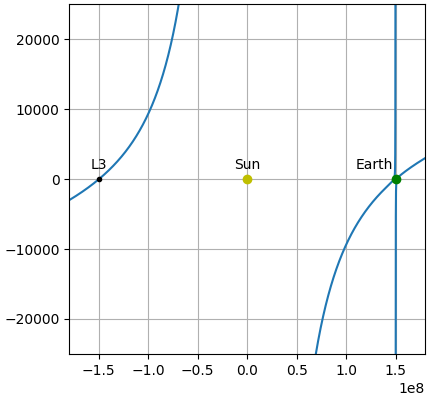
\includegraphics[scale=0.6]{r-accel-figure-1.png}
		\caption{\footnotesize Radial Acceleration between the Sun and Earth.}
		\label{fig:radial-accel-system}
	\end{subfigure}
	\hspace*{1cm}
	\begin{subfigure}[b]{0.4\textwidth}
		\centering
		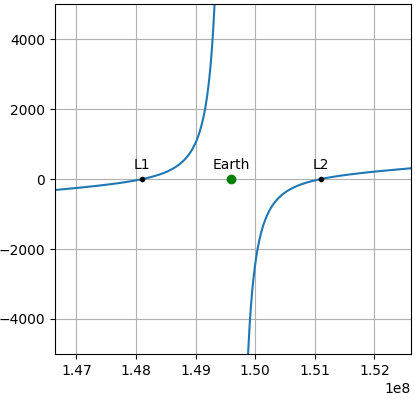
\includegraphics[scale=0.6]{r-accel-figure-2.png}
		\caption{\footnotesize Radial acceleration around the Earth.\vspace*{1.16em}}
		\label{fig:radial-accel-earth}
	\end{subfigure}
	\label{fig:radial-accel}
	\caption{Net acceleration of the Sun-Earth system. Graphs are created using \texttt{matplotlib}.}
\end{figure} % this figure can benefit from an explanation

%\begin{figure}[h!]
%	\centering
%	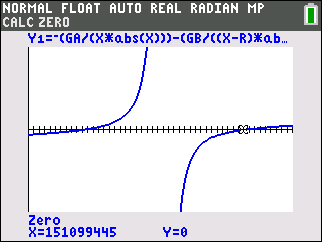
\includegraphics[scale=0.7]{accel-root.png}
%	\caption{Solution for L2 using a GDC.}
%	\label{fig:radial-l2}
%\end{figure}
Relative to the distance from the sun, the locations of the Lagrange points are as follows.
\begin{table}[h!]
	\centering
	\label{tab:lagrange-points}
	\caption{Distance of the collinear Lagrange points from the Sun}
	\vspace*{0.3cm}
	\begin{tabular}{|r|l|}
		\hline
		L1 & $1.481\times10^8 \si{\kilo\metre}$ \\
		\hline
		L2 & $1.511\times10^8 \si{\kilo\metre}$ \\
		\hline
		L3 & $-1.496\times10^8 \si{\kilo\metre}$ \\
		\hline
	\end{tabular}
\end{table}
	
	\section{Setup Scenarios for Equations of Motion}
	
	Using IB calculus, plus some vectors, we will be able to represent the motion of an object near a Lagrange point using equations.
It is important, however, that we first establish the system that we will be working with as well as restrictions that will make the mathematics slightly easier.
\begin{wrapfigure}{l}{0.6\textwidth}
	\centering
	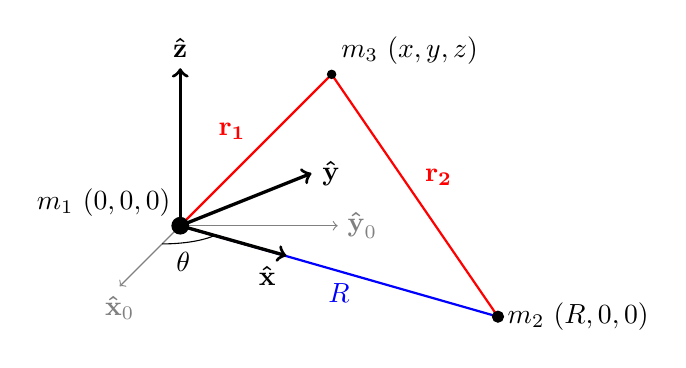
\begin{tikzpicture}
		\coordinate (o) at (0,0,0);
		\coordinate (m3) at (2.5,2.5,1.5);
		\coordinate (m2) at (5.19,0,3);
		\draw[thin,gray,->] (0,0,0) -- (0,0,2) node[below] {$\uvec{x}_0$};
		\draw[thin,gray,->] (0,0,0) -- (2,0,0) node[right] {$\uvec{y}_0$};
		
		\draw[thick,blue] (o) -- (m2) node[midway,yshift=-8pt]{$R$};
		\draw[thick,red] (o) -- (m3) node[midway,anchor=south east]{$\bvec{\bvec{r}_1}$};
		\draw[thick,red] (m2) -- (m3) node[midway,anchor=south west]{$\bvec{\bvec{r}_2}$};
		
		\draw[very thick,->] (0,0,0) -- (0,2,0) node[above] {$\uvec{z}$};
		\draw[very thick,->] (0,0,0) -- (1.73,0,0.99) node[below left] {$\uvec{x}$};
		\draw[very thick,->] (0,0,0) -- (1,0,-1.73) node[right] {$\uvec{y}$};
		
		\draw (0,0,0.6) arc [start angle=-90,end angle=-32,x radius=0.8,y radius=0.24];
		\node at (.5,0,1.2) {$\theta$};
		
		\filldraw (0,0,0) circle (3pt) node[above left] {$m_1$ $(0,0,0)$};
		\filldraw (m2) circle (2pt) node[right] {$m_2$ $(R,0,0)$};
		\filldraw (m3) circle (1.5pt) node[above right] {$m_3$ $(x,y,z)$};
	\end{tikzpicture}
	\vspace*{0.25cm}
	\caption{three-dimensional diagram of the Sun-Earth system with basis vectors relative to the Earth's orbit. Positions are exaggerated and not to scale.}
	\label{fig:3d-coords}
\end{wrapfigure}
Firstly, we must assert that $m_1 > m_2$, allowing the movement of the Sun due to the gravity of Earth is negligible.
This allows the Sun to be placed at the center of the coordinate system, avoiding the need to make considerations for the center of mass of the system.
It is also asserted that $m_2 > m_3$, so that, similarly to the previous assertion, the satellite has a negligible effect on Earth.
Secondly, continuing with the conditions from the previous calculations, it is assumed that the Earth is in a circular orbit, making the system a little easier to comprehend.
Thirdly, we assume that the orbit of the Earth has no inclination, meaning that it is co-planar to $\uvec{x}$ and $\uvec{y}$.
Lastly, and as shown in Figure \ref{fig:3d-coords}, we will have basis vectors $\uvec{x}$, $\uvec{y}$, and $\uvec{z}$ drawn relative to the orbit of the Earth, with initial vectors $\uvec{x}_0$, $\uvec{y}_0$, and $\uvec{z}_0$.
This is necessary to keep track of three dimensional space around the Lagrange points and also so that we can compose our equations of motion in terms of each dimension.
The satellite around L2, $m_3$, will have the coordinates $(x,y,z)$ represented by the vector $\bvec{r}$.

It is also important to acknowledge that we will need to take the derivative of vectors. Hence, let us assert that, for some vector \textbf{v} with the basis vectors $\uvec{i}$ and $\uvec{j}$ scalars $a$ and $b$:
\begin{equation*}
	\frac{d}{dt}\bvec{v} = \frac{da}{dt}\uvec{i} + \frac{db}{dt}\uvec{j} \text{.}
\end{equation*}
In other words, the derivative of a vector is equivalent to the derivative of its components.
This will allow us to analyze the movement of an object through kinematics in all three dimensions $x$, $y$, and $z$. Keep in mind that $\bvec{r}$---hence $x$, $y$, $z$, and $\theta$---are functions of time $t$ and we do not know how they are defined at this moment.

\newpage

One last thing: because we are dealing with vectors, Newton's law of gravitation can be rewritten in vector form:

\begin{equation*}
	\bvec{F} = m\bvec{a} = \frac{Gm_1m_2}{\|\bvec{r}\|^3}\bvec{r} \text{,}
\end{equation*}
where $r$ is the magnitude of $\bvec{r}$.

To start off, let us analyze our basis vectors.
We will use the notation $x'$ as the derivative of $x$ with respect to time $t$.
Because they are not actually static in the system ($\uvec{x}$ and $\uvec{y}$ rotate about the origin), their movement must be taken into account:
\begin{gather*}
	\uvec{x} = (\cos\theta)\uvec{x}_0 + (\sin\theta)\uvec{y}_0 \\
	\uvec{y} = (-\sin\theta)\uvec{x}_0 + (\cos\theta)\uvec{y}_0 \\
	\uvec{z} = \uvec{z}_0 \text{.}
\end{gather*}
Taking their first derivatives, we get:
\begin{gather*}
	\uvec{x}' = (-\sin\theta)\theta'\uvec{x}_0 + (\cos\theta)\theta'\uvec{y}_0 = \theta'\uvec{y} \\
	\uvec{y}' = -(\cos\theta)\theta'\uvec{x}_0 + (-\sin\theta)\theta'\uvec{y}_0 = -\theta'\uvec{x} \\
	\uvec{z}' = 0 \text{.}
\end{gather*}
And their second derivatives:
\begin{gather*}
	\uvec{x}'' = \theta''\uvec{y} + \theta'\uvec{y}' =  - \theta'^2\uvec{x} \\
	\uvec{y}'' = \theta''\uvec{x} - \theta'\uvec{x}' =  - \theta'^2\uvec{y} \text{.}
\end{gather*}
Given that this is uniform circular motion, $\theta'' = 0$.
%%%%%%%%%%%%%%%%%%%%%%%%%%%%%%%%%%%%%%%%%%%%%%%%%%%%%%%%%%%%%%%%%%%%%%
The position vector $r$ is expressed in unit vector form as:
\begin{equation*}
	\bvec{r} = x\uvec{x} + y\uvec{y} + z\uvec{z} \text{.}
\end{equation*}
We can take the second derivative of our position vector $\bvec{r}$ to find the acceleration.
\begin{equation*}
	\bvec{a} = \bvec{r}'' = (x\uvec{x})'' + (y\uvec{y})'' + (z\uvec{z})''
\end{equation*}
Our acceleration vector is then expanded to:
\begin{equation*}
	\bvec{a} = x''\uvec{x} + 2x'\uvec{x}' + x\uvec{x}'' + y'\uvec{y} + 2y'\uvec{y}' + x\uvec{y}'' + z''\uvec{z} + 2z'\uvec{z}' + z\uvec{z}'' \text{.}
\end{equation*}
\begin{samepage}
Substituting the derivatives of the basis vectors that we calculated earlier,
\begin{align}
	\bvec{a} &= x''\uvec{x} + 2x'(\theta'\uvec{y}) + x(- \theta'^2\uvec{x}) + y''\uvec{y} - 2y'(\theta'\uvec{x}) - x(\theta'\uvec{y}) + z''\uvec{z} \nonumber \\
	\bvec{a} &= \left(x'' - \theta'^2x - 2y'\theta'\right)\uvec{x} + \left(y'' + 2x'\theta' - \theta'^2y\right)\uvec{y} + z''\uvec{z} \label{eqn:accel-rotate} \text{.}
\end{align}
This equation represents the general centripetal acceleration of an object in circular motion in three dimensions.
To account for gravity, the acceleration due to gravity is expressed as:
\begin{align*}
	\bvec{F} = m_3\bvec{a} &= - \frac{Gm_1m_3}{\|\bvec{r}_1\|^3}\bvec{r}_1 - \frac{Gm_2m_3}{\|\bvec{r}_2\|^3}\bvec{r}_2 \\
	\bvec{a} &= - \frac{Gm_1}{\|\bvec{r}_1\|^3}\bvec{r}_1 - \frac{Gm_2}{\|\bvec{r}_2\|^3}\bvec{r}_2 \text{.}
\end{align*}
Where $\bvec{r}_1$ and $\bvec{r}_2$ is the distance of our satellite from $m_1$ and $m_2$, respectively.
$\bvec{r}_1$ and $\bvec{r}_2$ and their magnitudes, $\|\bvec{r}_1\|$ and $\|\bvec{r}_2\|$, are represented as:
\begin{align*}
	\bvec{r}_1 &= x\uvec{x} + y\uvec{y} + z\uvec{z} & \|\bvec{r}_1\| &= \sqrt{x^2 + y^2 + z^2} \\
	\bvec{r}_2 &= (x - R)\uvec{x} + y\uvec{y} + z\uvec{z} & \|\bvec{r}_2\| &= \sqrt{(x - R)^2 + y^2 + z^2} \text{.}
\end{align*}
Written in unit vector form, the acceleration vector can be expanded for each dimension:
\begin{equation*}
	\bvec{a} = \left(-\frac{Gm_1}{\|\bvec{r}_1\|^3}x - \frac{Gm_2}{\|\bvec{r}_2\|^3}(x - R)\right)\uvec{x} + \left(-\frac{Gm_1}{\|\bvec{r}_1\|^3}y - \frac{Gm_2}{\|\bvec{r}_2\|^3}y\right)\uvec{y} + \left(-\frac{Gm_1}{\|\bvec{r}_1\|^3}z - \frac{Gm_2}{\|\bvec{r}_2\|^3}z\right)\uvec{z} \text{.}
\end{equation*}
Now that it is written in terms of its components, just like Equation \eqref{eqn:accel-rotate}, we can set the components of each vector equal to each other.
\begin{align*}
	\uvec{x} : \qquad &x'' - \theta'^2x - 2y'\theta' = -\frac{Gm_1}{\|\bvec{r}_1\|^3}x - \frac{Gm_2}{\|\bvec{r}_2\|^3}(x - R) \\
	\uvec{y} : \qquad &y'' - \theta'^2y + 2x'\theta' = -\frac{Gm_1}{\|\bvec{r}_1\|^3}y - \frac{Gm_2}{\|\bvec{r}_2\|^3}y \\
	\uvec{z} : \qquad &z'' = -\frac{Gm_1}{\|\bvec{r}_1\|^3}z - \frac{Gm_2}{\|\bvec{r}_2\|^3}z
\end{align*}
The variables can then be rearranged to give us our equations of motion:
\begin{align}
	x'' &= \theta'^2x + 2y'\theta' -\frac{Gm_1}{\|\bvec{r}_1\|^3}x - \frac{Gm_2}{\|\bvec{r}_2\|^3}(x - R) \label{eqn:eomx}\\
	y'' &= \theta'^2y - 2x'\theta' -\frac{Gm_1}{\|\bvec{r}_1\|^3}y - \frac{Gm_2}{\|\bvec{r}_2\|^3}y \label{eqn:eomy}\\
	z'' &= -\frac{Gm_1}{\|\bvec{r}_1\|^3}z - \frac{Gm_2}{\|\bvec{r}_2\|^3}z \label{eqn:eomz}\text{.}
\end{align}
\end{samepage}

	
	\newpage
	
	\section{Deriving Equations of Motion}
	
	Equations \eqref{eqn:eomx}, \eqref{eqn:eomy}, and \eqref{eqn:eomz} are our equations of motion that govern the movement of a satellite around a Lagrange point.
Technically, we can use them to represent motion anywhere in our system, not just around the Lagrange points.

Notice how the equations of motion are similar to \eqref{eqn:x-accel1}, where the distance, velocity, and acceleration of each dimension can not be represented separately as functions of time.
Still, it is possible to make use of these equations through numerical approximation.
This means that, given some initial conditions (position and velocity), the output is calculated (acceleration) for a small interval of time.
Than, after letting the new output determine the rest of the system for the said time interval, the output is recalculated with the given change from the initial conditions.
Recursively, this is generally written as:

\begin{equation*}
	y_{n+1} = y_n + hf(t_n)
\end{equation*}

where $h$ indicates the length of the time interval and where some value $y_0$ is known.
This particular equation is known as ``Euler's method''\autocite{BrilEulers} and is used to approximate equations that are similar to our equations of motion.
The method used to approximate the equations of motion will not specifically be Euler's method, but its purpose is practically identical.

$G$, $R$, $m_1$, $m_2$, and $\theta'$ are known constants, with the latter defined as:

\begin{equation*}
	\theta' = \omega = \sqrt{\frac{G(m_1 + m_2)}{R^3}} \text{,}
\end{equation*}

meaning the unknown values to the equations of motion are $x, y, z, x', y'$, and $z'$.
By setting our initial $x$ coordinate $(1.511\times10^{11} - 10^3)\si{\metre}$, $1000\si{\metre}$ away from of L2, and the remaining conditions $y, z, x', y', z' = 0$, we can compute our first trajectory for our satellite, $m_3$.
As seen in Figure \ref{fig:3dplot1}, the satellite unremarkably falls back towards the Earth.
This makes sense since there is no initial velocity and the initial position places it in the influence of Earth's gravity.
\newpage
\begin{samepage}
\begin{figure}[ht!]
	\centering
	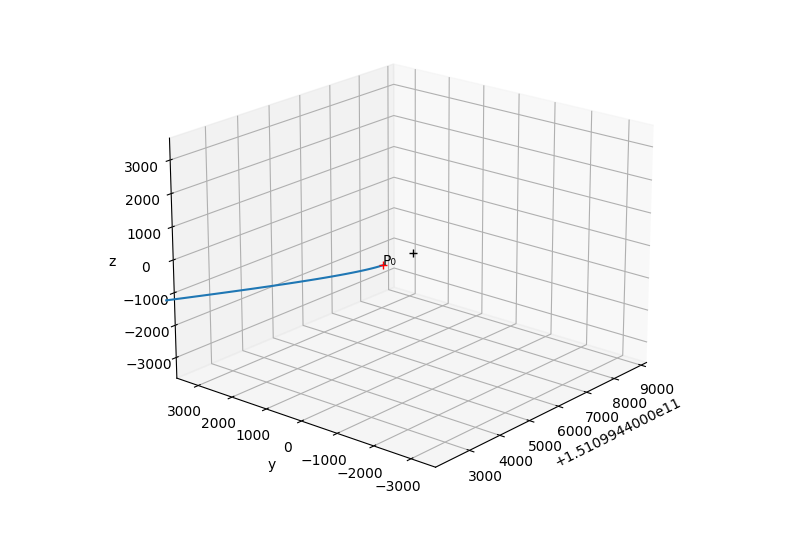
\includegraphics[scale=0.52]{3dplot1.png}
	\caption{Trajectory plot of an object near L2 fo the Sun-Earth system, x-coordinate is $(1.511\times10^{11} - 10^3)\si{\metre}$, all other conditions are 0.
		The red point, $P_0$, indicates the starting position of the object.
		The black point indicates the Lagrange point.
		Generated through the matplotlib Python library.
	}
	\label{fig:3dplot1}
\end{figure}
In order to create a trajectory that resembles an orbit, we need to apply velocity that is perpendicular to the acceleration to create circular motion.
Knowing that $v^2 = ar$, we can write the equation:
\begin{equation*}
	u_y = a\sqrt{x''r}
\end{equation*}
where $u_y$ is the initial velocity in the $y$ component and $a$ is the proportionality constant, assuming that the orbit being predicted is not circular.
After some trial and error, $a = 2.2$ makes for a good approximation.
\begin{figure}[H]
	\centering
	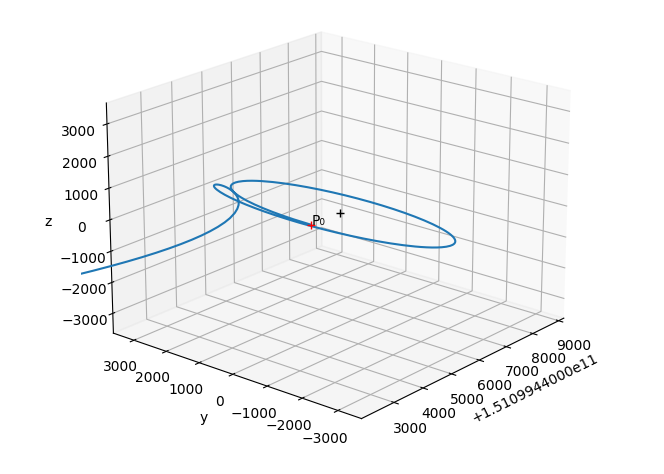
\includegraphics[scale=0.52]{3dplot2.png}
	\caption{Trajectory plot of an object $1000\si{\metre}$ in the proximity of L2 in the Sun-Earth system in a semi-stable halo orbit.}
	\label{fig:3dplot2}
\end{figure}
\end{samepage}
And would you look at that; in Figure \ref{fig:3dplot2}, it seems as if our satellite orbits nothing!
Of course, it is also seen that the satellite eventually falls out of its orbit, confirming the instability of collinear Lagrange points.

We can now use this model and compare it to the actual trajectory of objects orbiting Lagrange points.
Given that telemetry of the JWST is readily available through JPL Horizons System, we will use its orbit for comparison.
\begin{figure}[H]
	\centering
	\captionsetup[subfigure]{justification=centering}
	\begin{subfigure}[b]{0.4\textwidth}
		\centering
		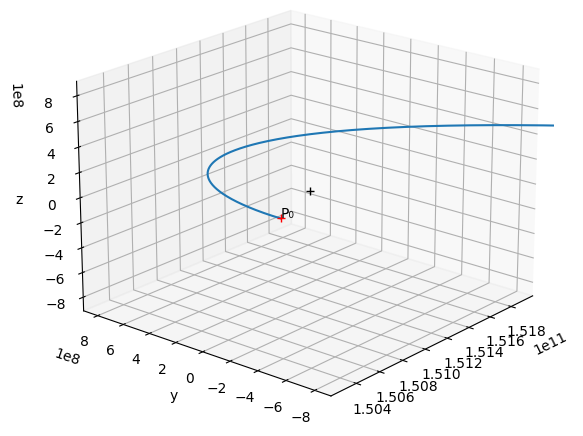
\includegraphics[scale=0.5]{3dplot3.png}
		\caption{Modelled trajectory plot of the JWST $2.5\times10^8\si{\metre}$ L2. Not modelled with station-keeping.}
		\label{fig:3dplot3}
	\end{subfigure}
	\quad
	\begin{subfigure}[b]{0.4\textwidth}
		\centering
		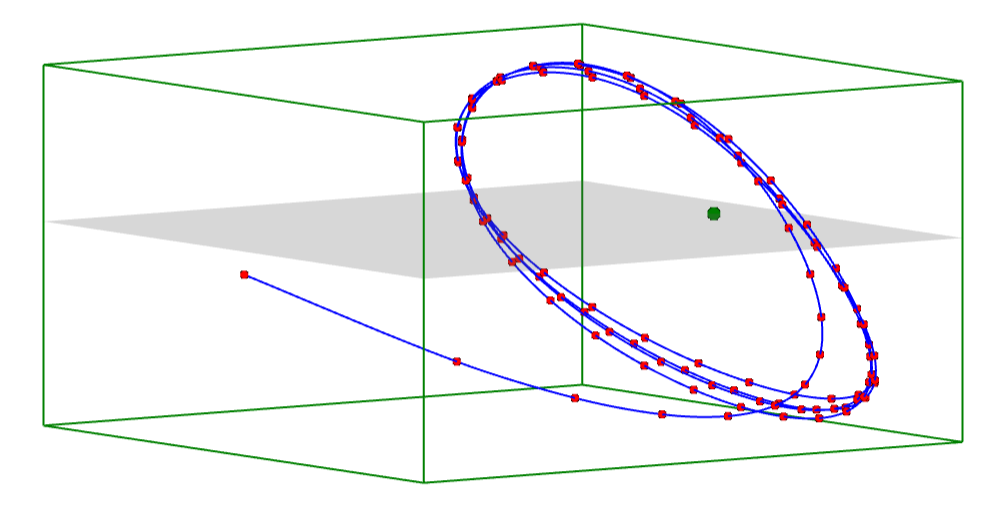
\includegraphics[scale=0.2]{xyjwstplot.png}
		\vspace*{1em}
		\caption{Trajectory of the JWST according to the JPL Horizons database.}
		\label{fig:3dplot4}
		\vspace*{1em}
	\end{subfigure}
	\caption{Trajectories of the JWST. Figure (a) has $P_0$ positioned at $(L_2 - 2.5\times10^8, 0, - 1.2\times10^8)$. Figure (b) generated through SageMath and produced by PM 2Ring on Stack Exchange.}
\end{figure}
Figure \ref{fig:3dplot3} is the trajectory of the JWST given the expected orbital characteristics prior to launch\autocite{JWSTHaloOrbit}.
Figure \ref{fig:3dplot4} is the trajectory of the JWST according to the JPL Horizons database from December 26th, 2021 to January 22, 2024\autocite{SEHaloOrbit}.
In Figure \ref{fig:3dplot3}, it is apparent that station-keeping, the use of onboard engines to stay on a specific orbit, is necessary for larger orbits around Lagrange points.
It is possible that a much more precise initial velocity approximations will produce a trajectory that stays in orbit for longer.
Still, the model seems to tend towards a similar elliptical, halo-like orbit that is shown in Figure \ref{fig:3dplot4}.
The difference in trajectories in both figures can be attributed to the degree of sophistication between our model and the model used by JPL.
This can include consideration for an elliptical, eccentric orbit of the Earth, the effects of the Moon's gravity, and orbital eccentricity of the JWST during its transfer to L2.
	
	\section{Plotting the Orbit}
	
	\section{Conclusion}
	
	\newpage
	
	\printbibliography[
	heading=bibintoc,
	title={References}
	]
	
\end{document}
